%%%%%%%%%%%%%%%%%%%%%%%%%%%%%%%%%%%%%%%%%%%%%%%%%%%%%%%%%%%%%%%%%%%%%%%%%%%%%%%
%
% THESIS DESCRIPTION:
%   A concise description of the main concepts of the thesis.
%
% RESEARCH:
%   A list of research activities which led to this thesis.
%
% EXPERIMENTS:
%   A list of the experiments performed which supported the research.
%
%%%%%%%%%%%%%%%%%%%%%%%%%%%%%%%%%%%%%%%%%%%%%%%%%%%%%%%%%%%%%%%%%%%%%%%%%%%%%%%
\documentclass[11pt,american]{report}
\usepackage{rit-thesis}
%%%%%%%%%%%%%%%%%%%%%%%%%%%%%%%%%%%%%%%%%%%%%%%%%%%%%%%%%%%%%%%%%%%%%%%%%%%%%%%
%   The following packages are all optional and depend on the specifics of what
% is contained in the thesis.  There is no harm in leaving them in.
%%%%%%%%%%%%%%%%%%%%%%%%%%%%%%%%%%%%%%%%%%%%%%%%%%%%%%%%%%%%%%%%%%%%%%%%%%%%%%%
\usepackage{subfigure}
\usepackage[refpages]{gloss}
\usepackage{babel}
\usepackage{times}
\usepackage{graphicx}
\usepackage{amssymb}
\usepackage{lscape}
\usepackage{verbatim}
\usepackage{enumerate}
\usepackage{afterpage}
\usepackage{float}

\floatstyle{boxed}
\newfloat{program}{tbhp}{lop}
\floatname{program}{Program}

%%%%%%%%%%%%%%%%%%%%%%%%%%%%%%%%%%%%%%%%%%%%%%%%%%%%%%%%%%%%%%%%%%%%%%%%%%%%%%%
%   Mark the document as 'draft' with a date. Be sure to comment this out for
% the final version.
\usepackage{watermark}
%\watermark{\hspace{-0.3in} \textbf{DRAFT} \hspace{2.0in} \textbf{\today}}
%%%%%%%%%%%%%%%%%%%%%%%%%%%%%%%%%%%%%%%%%%%%%%%%%%%%%%%%%%%%%%%%%%%%%%%%%%%%%%%

\makegloss

\begin{document}
%%%%%%%%%%%%%%%%%%%%%%%%%%%%%%%%%%%%%%%%%%%%%%%%%%%%%%%%%%%%%%%%%%%%%%%%%%%%%%%
% Title page
% The \title{} can contain line breaks as appropriate...
\title{\vspace{-0.20in}FTP-like Streams for the\\
   9P File Protocol}
% The \titleline{} must have no line breaks in it.
\titleline{FTP-like Streams for the 9P File Protocol}
% There should be no reason to change the \thesistype{} or the \MSThesistrue...
\thesistype{Thesis}
\MSthesistrue
% This date is really not used (unless \grantdate{}{} is blank)
\date{November 2010}
%%%%%%%%%%%%%%%%%%%%%%%%%%%%%%%%%%%%%%%%%%%%%%%%%%%%%%%%%%%%%%%%%%%%%%%%%%%%%%%

%%%%%%%%%%%%%%%%%%%%%%%%%%%%%%%%%%%%%%%%%%%%%%%%%%%%%%%%%%%%%%%%%%%%%%%%%%%%%%%
% AUTHOR
% The \author{} should be exactly the same as your diploma
    \author{John Floren}
    \dept{Computer Engineering}
%%%%%%%%%%%%%%%%%%%%%%%%%%%%%%%%%%%%%%%%%%%%%%%%%%%%%%%%%%%%%%%%%%%%%%%%%%%%%%%

%%%%%%%%%%%%%%%%%%%%%%%%%%%%%%%%%%%%%%%%%%%%%%%%%%%%%%%%%%%%%%%%%%%%%%%%%%%%%%%
% COMMITTEE MEMBERS
% The following information is for the signature page.
% Note that the definition for principal adviser uses two fields.
% This was needed so that the adviser's name could be placed on the
% abstract page without his/her title.
% \foursigstrue | \fivesigstrue but don't define BOTH to be true!!
    \principaladviser{Dr. Muhammad Shaaban}{Associate Professor}
    \advdept{Department of Computer Engineering}
    \firstreader{Dr. Roy Melton}{Lecturer}
    \firstdept{Department of Computer Engineering}
    \secondreader{Dr. Ron Minnich}{Distinguished Member of Technical Staff}%
    \seconddept{Sandia National Labs}
%%%%%%%%%%%%%%%%%%%%%%%%%%%%%%%%%%%%%%%%%%%%%%%%%%%%%%%%%%%%%%%%%%%%%%%%%%%%%%%% Use this only if \foursigstrue
%\thirdreader{Reader Three \\ Reader3 Title}
%\thirdreader
% Use this only if \fivesigstrue
%\fourthreader{Reader Four \\ Reader4 Title}
%%%%%%%%%%%%%%%%%%%%%%%%%%%%%%%%%%%%%%%%%%%%%%%%%%%%%%%%%%%%%%%%%%%%%%%%%%%%%%%

%%%%%%%%%%%%%%%%%%%%%%%%%%%%%%%%%%%%%%%%%%%%%%%%%%%%%%%%%%%%%%%%%%%%%%%%%%%%%%%
% This is the expected date that the committee will sign your thesis.
\grantdate{December}{2010}
%%%%%%%%%%%%%%%%%%%%%%%%%%%%%%%%%%%%%%%%%%%%%%%%%%%%%%%%%%%%%%%%%%%%%%%%%%%%%%%

%%%%%%%%%%%%%%%%%%%%%%%%%%%%%%%%%%%%%%%%%%%%%%%%%%%%%%%%%%%%%%%%%%%%%%%%%%%%%%%
% If you want to copyright your thesis / dissertation remove the line below.
\copyrightfalse% True by default
% The year of the copyright; usually same as the date the committee will
% sign the thesis. This won't be printed if \copyrightfalse
\copyrightyear{2010}
%%%%%%%%%%%%%%%%%%%%%%%%%%%%%%%%%%%%%%%%%%%%%%%%%%%%%%%%%%%%%%%%%%%%%%%%%%%%%%%

%%%%%%%%%%%%%%%%%%%%%%%%%%%%%%%%%%%%%%%%%%%%%%%%%%%%%%%%%%%%%%%%%%%%%%%%%%%%%%%
% This causes all front matter to be set.
\beforepreface%
%%%%%%%%%%%%%%%%%%%%%%%%%%%%%%%%%%%%%%%%%%%%%%%%%%%%%%%%%%%%%%%%%%%%%%%%%%%%%%%

%%%%%%%%%%%%%%%%%%%%%%%%%%%%%%%%%%%%%%%%%%%%%%%%%%%%%%%%%%%%%%%%%%%%%%%%%%%%%%%
% The dedication - if you choose to include one.
% It should be vertically centered in the page. Since the style format doesn't
% do it for you automatically, you can use the following technique.
\prefacesection{Dedication}
\vfill
\begin{center}
To my parents, Don and Donna Floren, for their constant support and patience through the course of my education.
\end{center}
\vfill
%%%%%%%%%%%%%%%%%%%%%%%%%%%%%%%%%%%%%%%%%%%%%%%%%%%%%%%%%%%%%%%%%%%%%%%%%%%%%%%

%%%%%%%%%%%%%%%%%%%%%%%%%%%%%%%%%%%%%%%%%%%%%%%%%%%%%%%%%%%%%%%%%%%%%%%%%%%%%%%
% The acknowledgements page - if you choose to include one.
% As in the dedication, it should be centered vertically in the page.
%
\prefacesection{Acknowledgments}
\vfill
\begin{center}
\indent I am grateful to Dr. Shaaban for working with me as my thesis advisor and Dr. Melton for joining my thesis committee. I would also like to thank Dr. Minnich for suggesting my thesis topic and providing invaluable support on some of the technical points of the work.

I am also grateful for the help and companionship of my fellow graduate students in the Computer Engineering department.
\end{center}
\vfill
%%%%%%%%%%%%%%%%%%%%%%%%%%%%%%%%%%%%%%%%%%%%%%%%%%%%%%%%%%%%%%%%%%%%%%%%%%%%%%%

%%%%%%%%%%%%%%%%%%%%%%%%%%%%%%%%%%%%%%%%%%%%%%%%%%%%%%%%%%%%%%%%%%%%%%%%%%%%%%%
%%  Collection of useful abbreviations.
\newcommand{\etc} {\emph{etc.\/}}
\newcommand{\etal}{\emph{et~al.\/}}
\newcommand{\eg}  {\emph{e.g.\/}}
\newcommand{\ie}  {\emph{i.e.\/}}
%%%%%%%%%%%%%%%%%%%%%%%%%%%%%%%%%%%%%%%%%%%%%%%%%%%%%%%%%%%%%%%%%%%%%%%%%%%%%%%

%%%%%%%%%%%%%%%%%%%%%%%%%%%%%%%%%%%%%%%%%%%%%%%%%%%%%%%%%%%%%%%%%%%%%%%%%%%%%%%
% Abstract
\begin{abstractpage}
The Plan 9 operating system from Bell Labs has broken a great deal of new ground in the realm of operating systems, providing a lightweight, network-centric OS with private namespaces and other important concepts. In Plan 9, all file operations, whether local or over the network, take place through the 9P file protocol. Although 9P is both simple and powerful, developments in computer and network hardware have over time outstripped the performance of 9P. Today, file operations, especially copying files over a network, are much slower with 9P than with protocols such as HTTP or FTP.

9P operates in terms of reads and writes with no buffering or caching; it is essentially a translation of the Unix file operations (open, read, write, close, \etc) into network messages. Given that the original Unix systems only dealt with files on local disks, it seemed that it may be necessary to extend 9P (and the file I/O programming libraries) to take into consideration the fact that many files now exist at the other end of network links. Other researchers have attempted to rectify the problem of network file performance through caching and other programmer-transparent fixes, but there is a second option. \emph{Streams} (a continuous flow of data from server to client) allow programmers to read and write data sequentially (an extremely common case) while reducing the number of protocol messages and avoiding some of the problems with round-trip latency. 

By adding streaming to the 9P protocol and extending the regular POSIX I/O functions, this work allows programmers to perform sequential file operations at speeds much closer to those of HTTP. Files are transferred using out-of-band TCP connections between the client and server. In tests, streaming allowed files to be transferred at equal or superior speeds to HTTP.
\end{abstractpage}
%%%%%%%%%%%%%%%%%%%%%%%%%%%%%%%%%%%%%%%%%%%%%%%%%%%%%%%%%%%%%%%%%%%%%%%%%%%%%%%

%%%%%%%%%%%%%%%%%%%%%%%%%%%%%%%%%%%%%%%%%%%%%%%%%%%%%%%%%%%%%%%%%%%%%%%%%%%%%%%
% Uncomment the line below if you don't want a list of tables to be printed.
% \tablespagefalse

% Uncomment the line below if you don't want a list of figures to be printed.
% \figurespagefalse

% \afterpreface generates the table of contents, list of tables (optional),
% and list of figures (optional).
\afterpreface%
%%%%%%%%%%%%%%%%%%%%%%%%%%%%%%%%%%%%%%%%%%%%%%%%%%%%%%%%%%%%%%%%%%%%%%%%%%%%%%%

\printgloss{Glossary}

%%%%%%%%%%%%%%%%%%%%%%%%%%%%%%%%%%%%%%%%%%%%%%%%%%%%%%%%%%%%%%%%%%%%%%%%%%%%%%%
% This is where the main body of the thesis starts
\body%
\chapter{Introduction}
Plan 9 from Bell Labs is a research operating system, originally conceived in the late 1980s with the aim of fixing the problems in UNIX\texttrademark \cite{Pike95:PBL}. Among other things, it features a single filesystem protocol, 9P, which is used to access all resources on the system, including control files for devices, the network stack, the windowing system, and the archival backup system. All of these files are made available by file servers, which are mounted to a namespace at the kernel level and then accessed using 9P messages.

However, while 9P provides a unified way to access the many devices and resources available on a Plan 9 system, it lacks in some aspects. 9P operates by sending a message requesting an operation, then waiting until the reply is received--it is, at its core, a synchronous process. In general, each 9P message sent corresponds to a function call made by the user program, making 9P a Remote Procedure Call (\gloss{RPC}) system. Although this is effective when used with local devices and file servers, it becomes problematic when dealing with file servers separated from the client by high-latency connections. Every read or write request must wait (with the process blocked) for the entire Round-Trip Time (RTT) between the client and server before any data comes back. With the rising prominence of the Internet, it has become apparent that accessing and transferring files from distant Plan 9 systems using 9P is extremely slow and inefficient, requiring far more time to complete a file transfer than the more popular Hyper-Text Transfer Protocol (\gloss{HTTP}) or File Transfer Protocol (\gloss{FTP}).

Where 9P operates in terms of ``chunks'' of a file, requested and delivered one piece at a time, HTTP and FTP deal with entire files at once. When a file is requested from an FTP server in passive mode, the FTP server and the client negotiate a separate, new TCP connection to be used to transfer the file all at once \cite{FTPrfc}. In HTTP, when a GET request is sent over the connection, the entire file is returned immediately (although a specific portion of the file can also be requested, which will also be sent immediately regardless of size) \cite{HTTPrfc}. Because FTP and HTTP push data directly to a TCP connection rather than waiting for it to be requested like 9P, they avoid many of the issues of latency.

This work proposes and implements a method for alleviating the latency problems in 9P. The solution, called ``streams'' in this text, operates by taking a leaf from FTP's book: it allows the creation of a new TCP connection to transfer file data. These streams, made available to programmers through library functions, can be used in any situation in which sequential reading or writing of a file occurs. Rather than attempting to improve performance with programmer-transparent adjustments behind the scenes, streams extend the POSIX-style file I/O API to put explicit control in the hands of the programmer. As the results show, the introduction of streams to 9P allows Plan 9 to transfer data using 9P just as quickly as with HTTP.

The rest of this document is structured as follows: Chapter 2 describes the background and motivation for this work, introducing Plan 9 and 9P, discussing the latency problem inherent in 9P (with measurements in comparison to HTTP), and presenting a condensed description of streaming 9P. Chapter 3 delves into previous work in the area of file protocol design, with particular attention paid to the problems of latency and bandwidth. Chapter 4 describes the high-level design of streaming 9P, explaining the programmer's interface to the system and the format of the 9P messages used to negotiate a stream. In Chapter 5, the actual implementation of streaming 9P is explained, showing how each part of the system (from user libraries to kernel functions) operates, and describing the compatibility functionality that was also included. Chapter 6 discusses the general methods for modifying user programs and 9P servers to use streams and explains how two specific programs, {\tt cp} and {\tt exportfs}, were modified in such a fashion. Chapter 7 contains the results obtained by testing streaming 9P, regular 9P, and HTTP at several different latencies and file sizes. Finally, Chapter 8 concludes the subject, analyzing the results and suggesting future areas of development.

\chapter{Background and Motivation}

This work deals with the Plan 9 operating system and its 9P protocol. To provide background on the work, this chapter describes the Plan 9 operating system, the 9P protocol, and the latency problem inherent in 9P. Initial tests, performed to get an idea of the issue, are discussed, and a solution to the problem is proposed.

\section{The Plan 9 Operating System}

Plan 9 is an operating system developed by AT\&T's Bell Labs beginning in the late 1980s \cite{Pike95:PBL}. In that time period, computers were beginning to move from large, expensive, monolithic devices which served many users to small, cheap graphical systems, which every person in an organization could have on their desks.

The UNIX\texttrademark operating system, also from Bell Labs, had been developed almost two decades earlier, in the time where hardware consisted of large, slow computers, text-only terminals, and little to no networking. Since its development it had been extended to run on microcomputers, network with other systems, and display bitmapped graphics. However, these additions came late and from a variety of sources. The original UNIX system had been tiny, tightly-designed, and rather consistent; the later additions made it much less so. Networking was added by using sockets, which behaved partially like files but not completely. The graphical user interface, in the form of the X Window System, was bulky, inefficient, and prone to crashing.

The designers of UNIX then decided it was time to begin again. Rather than fix UNIX, they began work on a new operating system, Plan 9. As Rob Pike said, ``The problems with UNIX were too deep to fix, but some of its ideas could be brought along'' \cite{Pike95:PBL}. Among the objectives of this new operating system were:

\begin{itemize}
	\item Access all resources as files.
	\item Use a standard protocol, 9P, to access these files.
	\item Allow resources to be joined and rearranged by each process in a single, private, hierarchical name-space.
\end{itemize}

Particular emphasis was also placed on networking, graphics, and overall simplicity. Development has continued at varying speeds over the past 20 years, through the first public release in the mid-1990s and the open-sourcing of the project in the early 2000s. Today, Plan 9 has a small but loyal following of developers and users who continue to improve and extend the project while remaining true to the original design mandates.

Having described the general background of Plan 9, it is useful to examine a few specific aspects of the system which will make subsequent explanation simpler. First, the general organization of computer networks under Plan 9 is described, and then a more detailed description of the 9P protocol is given.

\subsection{Organization of Plan 9 Networks}

Since Plan 9 was designed with networking and personal computers in mind, it exhibits a much more distributed nature than most operating systems. Plan 9 works best when used as a network of computers operating in different roles. The four basic roles are CPU server, auth server, file server, and terminal \cite{Pike95:PBL}. Figure \ref{figure:p9net} shows an example of a complex Plan 9 network, including CPU servers, file servers, and terminals.

\begin{figure}[h]
	\begin{center}
		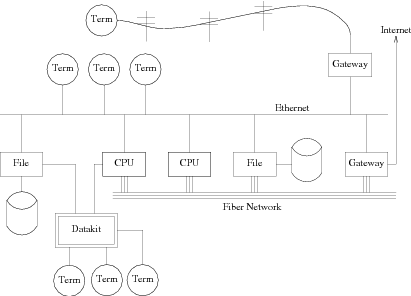
\includegraphics[width=0.75\textwidth]{p9net.png}
	\end{center}
	\caption{A Plan 9 network\cite{Pike95:PBL}}
	\label{figure:p9net}
\end{figure}

The purpose of a CPU server is to provide massive processing power when needed. CPU servers are typically the fastest, most expensive systems in a Plan 9 network, with high-end processors and large amounts of RAM. A CPU server might not have a hard drive at all, instead mounting the file system from the file server.

Auth servers provide authentication for the network. They store user information and passwords on a small disk and authenticate users who wish to access files on the file server, connect to the CPU server, \etc. Auth servers are generally small and low-power; the Sheeva Plug series of miniature computers, for example, have proven to be a popular choice as auth servers.

File servers are computers with large disk storage capacities, running disk-based file systems. Current file servers actually run two file systems, called \gloss{Fossil} and \gloss{Venti}. Venti is a block-based archival storage, while Fossil acts as the front-end to Venti. Typically, every day any new or changed data blocks are written to Venti and replaced in the Fossil storage with pointers to Venti blocks, which are never deleted. The two file systems in combination provide daily snapshots of the file tree, ensuring that important information can be retrieved if accidentally deleted. CPU servers, auth servers, and terminals all connect to the file server to store data.

Terminals are typically cheaper desktop PCs with large screens intended for direct use by users. The user works at a terminal, which mounts the file root from the file server after authenticating with the auth server. In this way, the same configuration and files are available to a user regardless of the actual terminal he may be using. If the processor or memory of the terminal prove insufficient, users of a terminal may use the {\tt cpu} command to execute commands on the CPU server (compilation, for example).

It is not strictly necessary to have all of these components as separate computers. It is quite common to have one system perform as a CPU, auth, and file server all at once; given the existence of a CPU server, it is not strictly necessary to have terminals, as users can also use the {\tt drawterm} program to connect directly to the CPU server and work on it.

All components of a Plan 9 network communicate using the 9P protocol, which is described in the following section.

\subsection{The 9P Protocol}
The Plan 9 operating system serves all file operations using the \gloss{9P} protocol. The contents of the local disk, the contents of removable media, remote file servers, and even device drivers such as the VGA and hard drive devices are accessed via 9P. It is essentially a network-transparent set of file operations.

In Plan 9, client programs access files using function calls in the C library, such as open, close, read, write, create, and stat. When a program calls one of these functions, the C library in turn generates an appropriate system call. Those system calls which operate on files in turn call functions in the appropriate kernel device depending on the file selected; in the case of files which exist on file servers (rather than generated in the kernel), the function call is translated into 9P messages and sent to the appropriate file server. 

9P messages come in pairs: a client sends a T-message (such as {\tt Tread}) and receives an R-message (such as {\tt Rread}) in response. The only exception is {\tt Rerror}, which may be sent in response to any T-message. A complete list of 9P messages is shown in Table \ref{table:9P} \cite{5intro}. Although there are not many 9P messages, the set of messages is sufficient to perform all file operations necessary to Plan 9.

\begin{table}[h]
\caption{Default 9P Messages}
\begin{center}
	\begin{tabular}{ | l | l | }
		\hline
		\bf{Message Name} & \bf{Function} \\ \hline
		Tversion/Rversion & Exchanges client/server 9P version numbers \\ \hline
		Tauth/Rauth & Authenticates client with server \\ \hline
		Rerror & Indicates an error (includes error string) \\ \hline
		Tflush/Rflush & Aborts a previous request \\ \hline
		Tattach/Rattach & Establishes a connection to a file tree \\ \hline
		Twalk/Rwalk & Descends a directory hierarchy \\ \hline
		Topen/Ropen & Opens a file or directory \\ \hline
		Tcreate/Rcreate & Creates a file \\ \hline
		Tread/Rread & Reads data from an open file \\ \hline
		Twrite/Rwrite & Writes data to an open file \\ \hline
		Tclunk/Rclunk & Closes an open file \\ \hline
		Tremove/Rremove & Removes a file \\ \hline
		Tstat/Rstat & Requests information about a file \\ \hline
		Twstat/Rwstat & Changes information about a file \\ \hline
	\end{tabular}
\end{center}
\label{table:9P}
\end{table}

All connections are initiated with the exchange of a {\tt Tversion/Rversion} pair. In this exchange, the client and server insure that they are both speaking a compatible version of the 9P protocol. At the time of writing, the most recent version was called ``9P2000'', with an earlier version ``9P'' long deprecated. If either the client or the server returns a version that the other does not understand, no communication can be performed.

Once the protocol version has been established, a client typically sends a {\tt Tattach} message to attach to a specific file tree. Then, the client is free to {\tt Twalk}, {\tt Tstat}, {\tt Topen}, \etc all over the file tree.

When a user opens a file, the client program makes an {\tt open()} system call, which is translated into a 9P message, {\tt Topen}, which is sent to the file server. The file server responds with an {\tt Ropen} message when the file has been opened. The client then sends {\tt Tread} and {\tt Twrite} messages to read and write the file, with the server responding with {\tt Rread} and {\tt Rwrite}. When the transaction is completed, the client sends {\tt Tclunk} and receives {\tt Rclunk} in return, at which point the file is closed.

Although 9P is a very simple protocol which works well for many uses, it does have disadvantages. The next section describes the disadvantage of interest to this work and compares 9P's performance to that of HTTP.

\section{Motivation}
The T-message/R-message model of 9P is conceptually very simple. Data are sent only when requested by the client; there is no read ahead, buffering, or inherent caching. In 1995, when files were small and networks tended to be local within an organization, this was not a problem. Today, files may regularly stand in the range of gigabytes. Large files are very frequently transferred over high-latency networks, such as a trans-continental Internet link.

Anecdotal evidence indicates that downloading a file from a Plan 9 server to a Plan 9 client using 9P is several times slower than downloading the same file via HTTP. If a large file is being transferred from one Plan 9 system to another using 9P, it is often faster to cancel the transfer half-way through, move the file to the httpd directory, and download it over http instead. 

Another example is the simple case of playing an MP3 file from a remote machine. If the file is accessed via 9P, playback stutters every few seconds, because the player application issues read calls for the next chunk of the file and runs out of audio to play while it is still waiting for the new chunk to arrive. If, however, the file is fetched via HTTP and piped to the music player ({\tt "hget http://server/file.mp3 | games/mp3dec"}), playback continues smoothly.

The performance of 9P is also of interest in the use of Plan 9 on supercomputers, where it is essential to be able to transfer data quickly. Supercomputing operations in particular must distribute large amounts of information to a large number of nodes as quickly as possible. While the internal networks of supercomputers have extremely low latency, the use of {\tt Tread/Rread} pairs adds to the congestion of the network, injuring performance. Using streams to transfer data sets and executable programs between supercomputer nodes could have a huge impact on the time a computation takes, in a field where small delays add up fast.

\subsection{Initial Testing}
With this in mind, a number of tests were made to compare the transfer speeds of HTTP and 9P. Two Plan 9 computers, one running as a CPU/auth/file server and one running as a standalone terminal, were connected via a network consisting of a 100 Mbit switch and a 10 Mbit hub, with a Linux computer acting as a gateway between the switch and the hub. The Linux computer was configured using the {\tt netem} kernel extensions to induce delay between the two halves of the network. The use of a 10 Mbit hub served to reduce the available bandwidth, which in combination with the artificially-induced latency was intended to resemble an Internet connection. Figure \ref{figure:network} illustrates the testing setup used. The testing procedure used is also described more thoroughly in the Results section of this document.

\begin{figure}[h]
	\begin{center}
		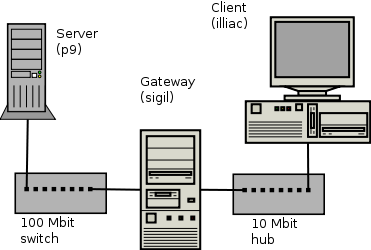
\includegraphics[width=0.75\textwidth]{network.png}
	\end{center}
	\caption{Local network for simulating latency}
	\label{figure:network}
\end{figure}

The tests consisted of using 9P and HTTP to transfer several randomly-generated files across the network. Files sized 10 MB, 50 MB, 100 MB, and 200 MB were used. The Linux bridge was set to provide three different round-trip latencies for the three different tests: no induced latency (approx. 500 $\mu$s round trip), 15 ms latency, and 50 ms latency.

\begin{table}[h]
	\caption{HTTP vs. 9P, no induced latency, average RTT 500 $\mu$s}
	\begin{center}
		\begin{tabular}{ | c || r | r | }
			\hline
			\bf{File Size (MB)} & \bf{9P (sec.)} & \bf{HTTP (sec.)} \\ \hline
			10 & 10.60 & 11.91 \\ \hline
			50 & 51.96 & 62.04 \\ \hline
			100 & 103.64 & 124.80 \\ \hline
			200 & 208.81 & 249.50 \\ \hline		
		\end{tabular}
	\end{center}
	\label{table:nolatency}
\end{table}

\begin{figure}[h]
	\begin{center}
		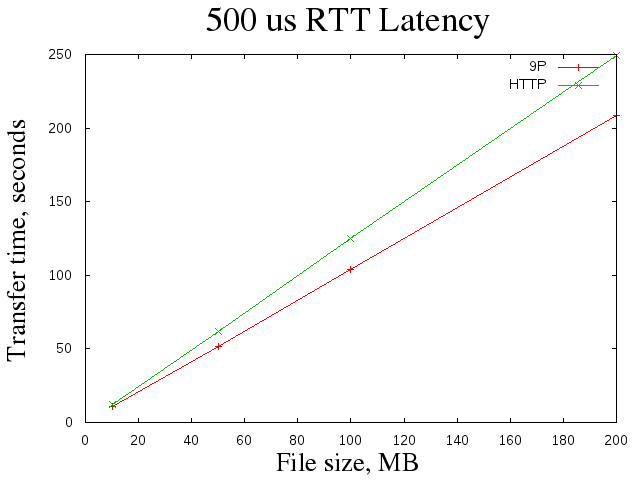
\includegraphics[width=0.75\textwidth]{500us.png}
	\end{center}
	\caption{HTTP vs. 9P, 500 $\mu$s RTT}
	\label{figure:500us}
\end{figure}

As Table \ref{table:nolatency} and Figure \ref{figure:500us} show, there was very little difference between 9P and HTTP when latency was low--in fact, 9P slightly outperformed HTTP. This behavior is desirable and should be preserved in any modifications.

\begin{table}[h]
	\caption{HTTP vs. 9P, induced latency of 15 ms RTT}
	\begin{center}
		\begin{tabular}{ | c || r | r | }
			\hline
			\bf{File Size (MB)} & \bf{9P (sec.)} & \bf{HTTP (sec.)} \\ \hline
			10 & 29.57 & 14.08 \\ \hline
			50 & 147.44 & 70.81 \\ \hline
			100 & 296.06 & 140.38 \\ \hline
			200 & 590.94 & 281.63 \\ \hline		
		\end{tabular}
	\end{center}
	\label{table:15mslatency}
\end{table}

\begin{figure}[h]
	\begin{center}
		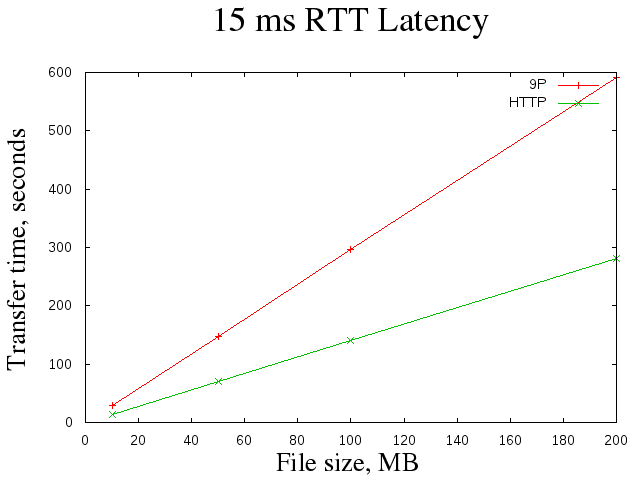
\includegraphics[width=0.75\textwidth]{15ms.png}
	\end{center}
	\caption{HTTP vs. 9P, 15 ms RTT}
	\label{figure:15ms}
\end{figure}

However, when 7.5 ms of latency was introduced in each direction (total RTT of 15 ms), 9P fell badly behind (see Table \ref{table:15mslatency} and Figure \ref{figure:15ms}). While HTTP took only 1.13 times as long to copy a 200 MB file with 15 ms RTT versus 500 μs RTT, 9P took 2.83 times as long.

\begin{table}[h]
	\caption{HTTP vs. 9P, induced latency of 50 ms RTT}	
	\begin{center}
		\begin{tabular}{ | c || r | r | }
			\hline
			\bf{File Size (MB)} & \bf{9P (sec.)} & \bf{HTTP (sec.)} \\ \hline
			10 & 76.16 & 19.43 \\ \hline
			50 & 374.07 & 98.88 \\ \hline
			100 & 747.13 & 197.90 \\ \hline
			200 & 1512.31 & 400.00 \\ \hline		
		\end{tabular}
	\end{center}
	\label{table:50mslatency}
\end{table}

\begin{figure}[h]
	\begin{center}
		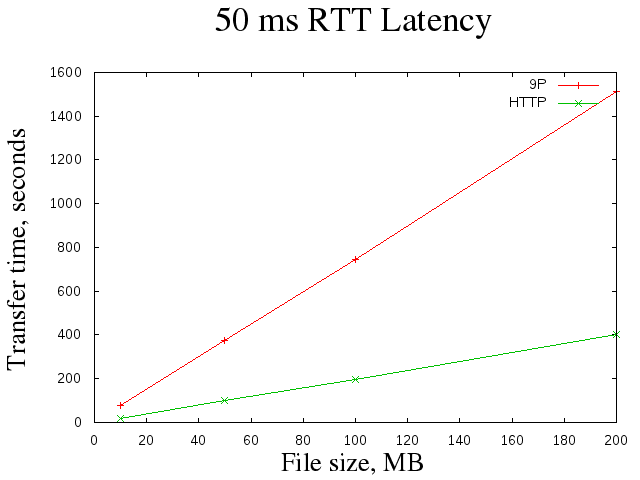
\includegraphics[width=0.75\textwidth]{50ms.png}
	\end{center}
	\caption{HTTP vs. 9P, 50 ms RTT}
	\label{figure:50ms}
\end{figure}

Table \ref{table:50mslatency} and Figure \ref{figure:50ms} show the results of the final test, with a RTT of 50 ms. Note that it took HTTP about 250 seconds to copy a 200 MB file with no induced latency, and required less than twice that time (400 seconds) to copy the same file with 25 ms of latency in each direction. 9P, on the other hand, went from a speedy 208 seconds to about 1,512 seconds--over 25 minutes.

Given that latencies on the Internet can easily reach or surpass the times tested here---at the time of writing, the RTT from Rochester, NY to Livermore, CA was around 90 ms---it became clear that 9P was not suitable for transferring data across the Internet. The gap between standard 9P and HTTP increases with latency; since the speed of light imposes a certain latency on all operations, 9P had to be modified to achieve better performance in a world where files may increasingly be stored thousands of miles away.

Having illustrated the latency problem inherent in 9P in this section, the next section discusses the method by which this work proposes to alleviate that problem---streams.

\section{Streams for 9P}

The primary reason for 9P's poor performance over high-latency network connections is the \gloss{RPC} nature of 9P. When a program wishes to read a piece of a file from a remote server, it must send a {\tt Tread} message, and then wait for the server to reply with an {\tt Rread}, as illustrated in Figure \ref{figure:9pmodel}. The program ends up blocked for twice the latency of the network connection; in the meantime, it accomplishes nothing. As the tests in the previous section showed, this is acceptable over local networks, but rapidly becomes problematic over even the fastest Internet links.

\begin{figure}[h]
	\begin{center}
		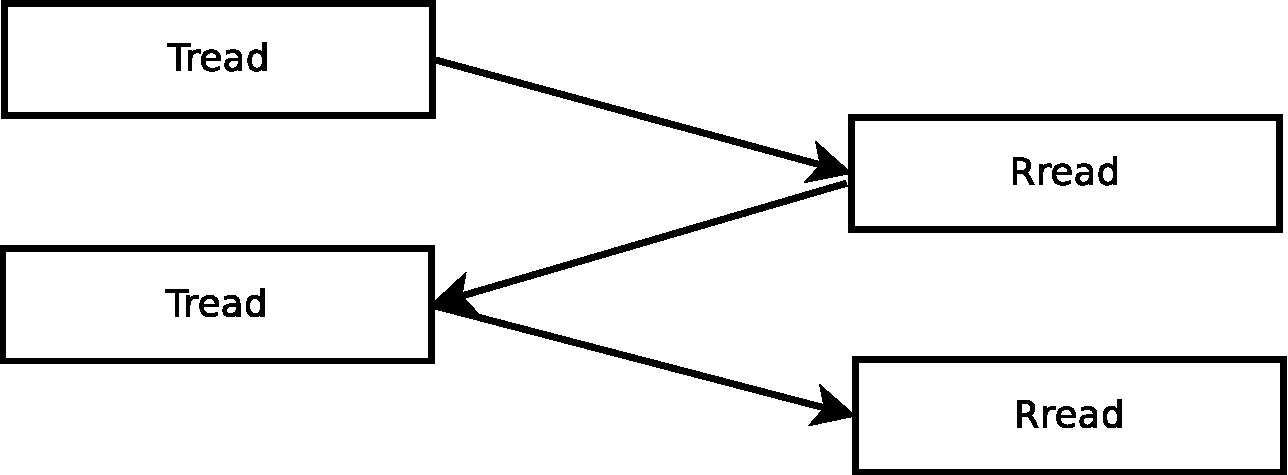
\includegraphics[width=0.75\textwidth]{9P-read.pdf}
	\end{center}
	\caption{The 9P file reading model}
	\label{figure:9pmodel}
\end{figure}

Many programs operate on files in a simple sequential manner. For instance, the {\tt cp} program reads 8 kB at a time from the source file and writes it out to the destination file. Editors read in files from start to finish; audio and video players start at the beginning of a file and continually read through it as they play. Therefore, it makes sense to consider the sequential case for optimization.

When a file is read in a purely sequential fashion, it becomes unecessary to specify the next offset into the file from which to read. The next read always takes the bytes directly following the first read. In its unmodified state, 9P makes absolutely no concession to the case of sequential file reading or writing; it requires a specific offset to be specified every time a file is read or written, and it will never send data that is not specifically requested by a {\tt Tread} message.

In considering the specific case of 9P, it became evident that an entire file could be read sequentially without sending {\tt Tread} requests each time a program needed the next piece of data. In fact, sequentially reading the entire file could be accomplished by sending a single request, then receiving the whole file at once, which is the model HTTP and FTP utilize (see Figure \ref{figure:httpmodel}).

\begin{figure}[h]
	\begin{center}
		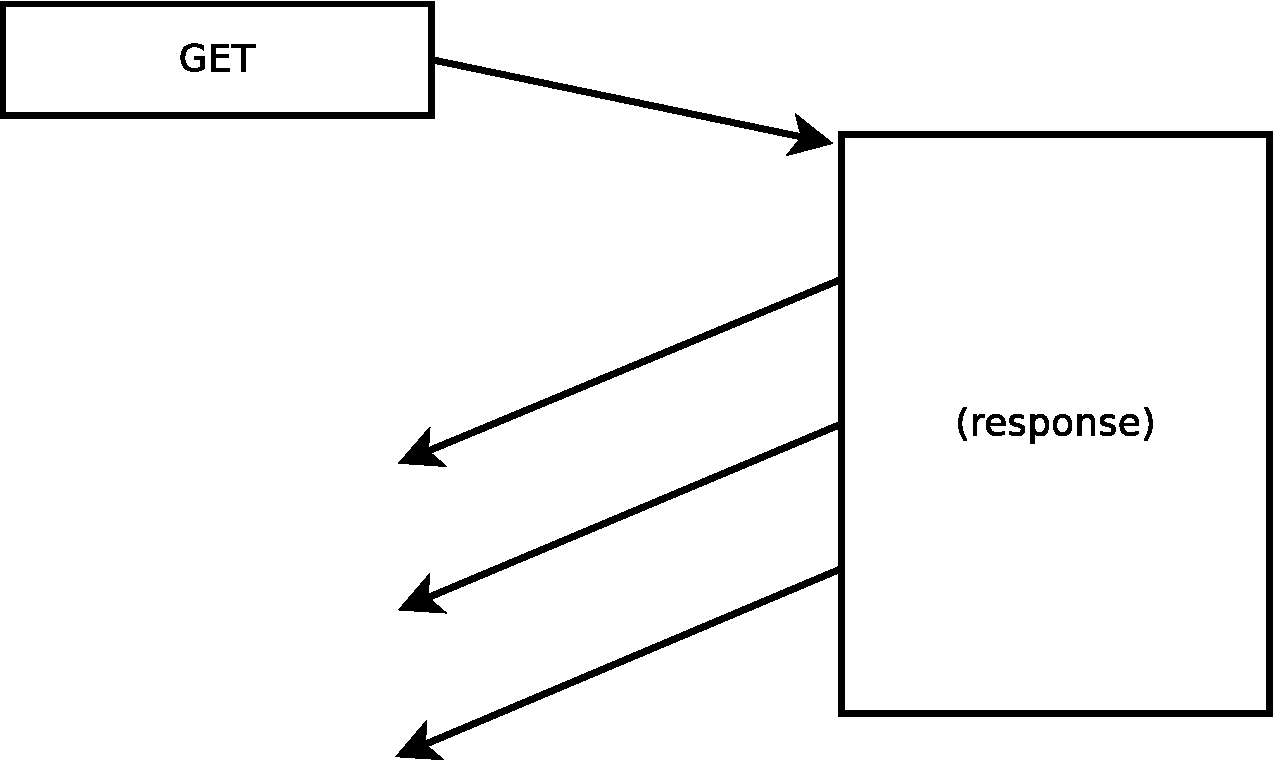
\includegraphics[width=0.75\textwidth]{HTTP-get.pdf}
	\end{center}
	\caption{The HTTP file reading model}
	\label{figure:httpmodel}
\end{figure}

To improve the performance of sequentially reading files over a 9P connection, it was determined that a new style of file interaction would be implemented, called {\emph streams}. A stream is a separate \gloss{TCP} connection opened specifically to transfer a single file, very similar to FTP's passive mode. Streams are negotiated using 9P messages over the existing 9P connection, but actual data transfer takes place out-of-band over the TCP connection rather than the shared 9P connection.

Although the possibility of converting Plan 9 to use HTTP rather than 9P was considered, it was rejected for several reasons. First, completely replacing 9P with HTTP would require significantly more work, as 9P is thoroughly integrated into the entire system. Second, 9P is better suited for use with Unix-style file systems, while HTTP is primarily for serving mostly static files to web browsers and other similar clients.

As the next chapter shows, using streams to improve performance over high-latency connections is a departure from most other file protocol work. In general, previous researchers have focused primarily on finding ways to improve the performance of the protocol transparently so as not to require any changes in applications; some of these efforts are discussed and contrasted to streaming 9P.

\chapter{Previous Work}
File system performance over low-bandwidth and high-latency links has been an area of concern for decades. Many researchers have worked to improve performance using caching, while others have taken different approaches, looking to reduce protocol overhead or adopt new, more effective methods.

\section{Parallel {\tt cp}}
One early attempt at solving the problem of high-latency 9P file transfers was the {\tt fcp} program \cite{1cp}. Since a process that reads or writes a file must wait in the blocked state until the reply comes back from the server, {\tt fcp} starts multiple processes to fetch and write data concurrently . The source file is divided into {\emph n} sections and a process is forked for each section. Each process then reads its section from the source file and writes it to the appropriate part of the destination file.

Although {\tt fcp} provides a significant performance improvement when copying large files over high-latency network connections, its multi-process approach is too complex. It should not be necessary to implement multiple processes simply to read a file.

\section{FTP}
The File Transfer Protocol, FTP, is one of the earliest networked file protocols. Its primary use is to transfer files between computers, rather than allow read/write access to remote files. In the context of this work, its most salient feature is its passive mode. In passive mode, when a client requests a file, the server replies with a TCP port. The client then connects to the port and retrieves the file data through the resulting connection \cite{FTPrfc}.

FTP's passive mode is very similar to the streaming extension proposed in this work. The primary difference is that 9P is designed as a more general file access protocol, with the streaming extension providing a method for reading and writing files sequentially while maintaining the generality of the rest of 9P.

\section{Op}
In 2007, Francisco Ballesteros et. al. \cite{Op} presented their work on a high-latency system. Their ongoing project is called Octopus, a distributed system built on top of Inferno, which in turn is derived from Plan 9. A replacement for the 9P protocol was written which combines several file operations into two operations, {\tt Tput/Rput} and {\tt Tget/Rget}. Thus, a client may send a single {\tt Tget} request to open a file, get the metadata, and read some of the data.

The Op system was implemented using a user-mode file server, Oxport, and a user-mode client, Ofs. Oxport presents the contents of a traditional 9p-served file tree via Op. Ofs then communicates with Oxport using Op; Ofs provides the exported file tree to clients on the local machine. When a user program, such as cat, attempts to read a file that actually resides on a remote machine, the 9P commands are sent to Ofs. Ofs then attempts to batch several 9P messages into a single Op message; a call to {\tt open()} normally sends {\tt Twalk} and {\tt Topen} messages, but Ofs will batch them both into a single {\tt Tget} message to walk to the file, open it, and fetch the first {\tt MAXDATA} bytes of data. Metadata from files and directories is also cached locally for the duration of a ``coherency window'' in the interest of reducing network read/writes while not losing coherency with the server file system.

The Op protocol showed significant reductions in program run-time latency. An {\tt lc} (equivalent to {\tt ls}) that originally took 2.3 seconds to complete using original 9P took only 0.142 seconds with a coherency window of 2 seconds. The bandwidth was improved by orders of magnitude when building software using {\tt mk}.

While Op gave good results, its design is not optimal. The Op protocol is only spoken by Oxport and Ofs. As user-level programs, they incur more overhead than in-kernel optimizations. Also, when the functionality is implemented as a transparent operation, it does not allow the programmer to choose between traditional 9P-style operations and Op; a separate streaming system would give that additional flexibility. Op also saw poorer performance than regular 9P on low-latency links, which are the norm in supercomputers; as Plan 9 expands into supercomputing and across the global Internet, it needs an improved 9P protocol that can work well over both high- and low-latency connections. Finally, Op was optimized for small files, having a relatively small {\tt MAXDATA} (the amount of data that can be transferred in one Rget message). Op would still need to execute many {\tt Tget} requests to transfer a large file, which is one of the cases of interest in this thesis.

\section{NFS}
The NFS protocol version 4 utilizes a similar strategy to Op with its COMPOUND RPCs, which allow clients to batch up several \gloss{RPC}s into one message. Thus, a client could read from a file in one RPC by sending a LOOKUP, OPEN, and READ all in a single COMPOUND RPC \cite{NFS4}. Although this helps with the latency problem, clients would still have to issue multiple READ commands to fetch the entirety of a large file, at which point latency issues would arise again.

NFS 4 also implements a feature called open delegations, which allows a client computer to manage open and close requests locally. Essentially, the server delegates control over a file to the client. Programs on the client can open, close, read or write the file without the client being required to write back the changes when the programs close the file. This means that a file can be read, written, and read back multiple times without as much data flushing as would normally occur, avoiding performance problems when the connection to the server has high latency. However, as the NFS specification illustrates, the semantics of open delegations are complex; the streaming extensions to 9P are singificantly simpler.

\section{HTTPFS}
Oleg Kiselyov in 1999 presented a paper \cite{HTTPFS} describing his work on a file system based on HTTP. This file system, HTTPFS, is capable of reading, writing, creating, appending, and deleting files using only the standard {\tt GET, PUT, HEAD,} and {\tt DELETE} requests.

The HTTPFS consists of two components, a client and a server. The client can in fact be any program which accesses files; such a program is converted to an HTTPFS client by linking with a library providing HTTPFS-specific replacements for the regular file system calls, such as open, read, close, \etc. These replacement functions simply call the standard system calls, \emph{unless} the filename given begins with {\tt http://}. If a URI is given, the function instead creates an appropriate HTTP request and sends it to the server. For example, calling:

{\scriptsize{\tt open("http://hostname/cgi-bin/admin/MCHFS-server.pl/README.html", O\_RDONLY)}} \cite{HTTPFS}

\noindent causes the client to send out a {\tt GET} request for that file. When the file is received, the client caches it locally; reads and writes then take place on the locally cached copy.

Kiselyov wrote an example HTTPFS server, called MCHFS. MCHFS acts much like a regular web server, allowing any browser to get listings of files. However, it also allows the user to access the entire server filesystem under the path component {\tt DeepestRoot}, for example: 

{\scriptsize{\tt open("http://hostname/cgi-bin/admin/MCHFS-server.pl/DeepestRoot/etc/passwd", O\_RDONLY)}}. \cite{HTTPFS}

An interesting factor of the HTTPFS design is its approach toward caching and concurrency. When a file is opened, the entire file is fetched via HTTP and cached locally. All reads and writes to that file then take place on the local copy. Finally, when {\tt close()} is called, the local copy is written back to the server using {\tt PUT}.

In some ways, HTTPFS is quite similar to the goal of this thesis. It reads the entire remote file at once and then redirects reads and writes to the local copy. However, as with Op, it does not give the user any choice: all HTTP-served files are read all at once and cached locally, while all other files are accessed traditionally. The goal of 9P streams is to allow the programmer a clear choice in accessing files, either by the traditional open/read/write methods, or using streams.

\section{LBFS}
The Low-Bandwidth File System (LBFS) adapted typical caching behavior for low-bandwidth operations \cite{LBFS}. The most salient change was the use of hash-indexed data chunks. LBFS clients maintain a large local file cache; files are divided into chunks and indexed by a hash. These hashes are then used to identify which sections of a file have been changed and avoid retransmitting unchanged chunks. When reading a file, the client issues a GETHASH request to get the hashes of all chunks in the file, then issues READ RPCs for those chunks which are not already stored locally. This technique provided excellent results but the entire premise is rapidly becoming far less important; bandwidth is rarely a problem today. LBFS made no provisions to account for latency, which remains a problem over long links due to the limitations of switching technology and the speed of light.

\section{Transparent Informed Prefetching}
Patterson, Gibson, and Satyanarayanan in 1993 experimented with the use of Transparent Informed Prefetching (TIP) to alleviate the problems of network latency and low bandwidth. With TIP, a process informs the file system of its future file accesses. For instance, the {\tt make} program prepares a directed acyclic graph of dependencies, including files; this list of files would be sent to the filesystem for pre-fetching. In testing, separate processes were used to perform pre-fetching from local disks and Coda file servers. Results showed significant (up to 30\%) reduction in execution times for programs such as {\tt make} and {\tt grep} \cite{TIP}.

\section{Parallel File Systems}
Other researchers have applied parallelism to the task \cite{Lee01appliedtechniques,PVFS}. Filesystems such as PVFS stripe the data across multiple storage nodes; a client computer then fetches chunks of files from several different computers simultaneously, reducing the impact of latency and the bottleneck of bandwidth to some extent. Others \cite{NFSP} spread data across the disks of the client nodes and index it using a metadata server.

A simple parallel file transfer program already exists in Plan 9: the fcp program uses several threads, each copying its own portion of the file---but it is unreasonable to expect every program to implement multi-threaded file reading to cover the holes in 9P. Parallel file systems in general are frequently not an option; often, only one computer is available to serve files. The complexity of coordinating multiple servers and having the client deal with all of these servers makes a simpler solution desirable.

\section{Summary}
Clearly, while caching and other file system modifications have been successful, the general theme has been one of operating in a user-transparent fashion. The results of this is that behavior can sometimes be unclear, unexpected, or inconvenient (cache coherency problems, \etc). By providing a clear choice to the programmer, such problems can be avoided, allowing the programmer to choose streams where high-speed sequential reads are necessary and traditional I/O elsewhere. The next chapter describes the interface that is provided to the programmer and the 9P message formats which are used to set up a stream.

\chapter{Streaming 9P Design}

In the previous chapter, other attempts to improve file protocol performance over high latency connections were described. Some found success by grouping messages, while others performed transparent pre-fetching and caching. However, rather than use a transparent method for improving performance, this work uses an explicitly-requested external transfer method, called streaming.

As described in an earlier section, streams are separate TCP connections used to transfer file data sequentially. The client requests a stream using a new 9P message, {\tt Tstream}, and the server replies with an IP address and a TCP port. The file is then transferred out-of-band over the TCP connection, allowing for higher transfer rates.

The high-level design of the streaming extension for 9P can be described in two parts. The first is the set of functions by which programmers use streaming, and the second is the actual format of the 9P messages sent between the client and the server; both parts are described in this chapter. Finally, an earlier, rejected design is discussed. Actual implementation details are described in the next chapter.

\section{Library Interface}

Streams are made available to the programmer through the C library, {\tt libc}. There are two ways in which programmers may use streams: in a regular (client) program, or in a file server.

Regular programs such as {\tt cp} or an MP3 player utilize streams using the library functions {\tt stream}, {\tt sread}, {\tt swrite}, and {\tt sclose}. These routines initialize a stream, read from a stream, write to a stream, and close a stream, respectively, and are shown in Table \ref{table:libfunc}. The functions use a data structure called Stream, shown below.

\begin{table}[h]
	\caption{Streaming Library Function Prototypes}
	\begin{center}
		\begin{tabular}{ | c | }
			\hline
			{\tt Stream* stream(int fd, vlong off, char isread)} \\ \hline
			{\tt long sread(Stream* s, void *buf, long n)} \\ \hline
			{\tt long swrite(Stream* s, void *buf, long n)} \\ \hline
			{\tt int sclose(Stream* s)} \\ \hline
		\end{tabular}
	\end{center}
	\label{table:libfunc}
\end{table}

\begin{program}
\begin{verbatim}
typedef struct Stream {
  int ofd;            // The underlying file being streamed
  int conn;           // The TCP connection
  char *addr;         // The server's IP and port
  vlong offset;       // Current offset into the file
  char isread;        // Read/write flag
  char compatibility; // Compatibility mode flag
} Stream;
\end{verbatim}
\caption{Stream data structure}
\end{program}

The {\tt stream} function serves to initialize a stream. It takes as arguments a file descriptor, a file offset, and a flag to indicate if the stream should be for reading or writing. The function operates on a file which has already been opened using the {\tt open} call. {\tt stream} is the only function which required a new system call, as described in the Implementation section. It returns a structure containing the underlying file descriptor, a file descriptor pointing to the TCP stream which was established, a string containing the address of the server, the current read/write offset in the file (used for compatibility), a flag describing the stream as read or write type, and a flag indicating if the stream should be used in compatibility mode.

Reading from a stream is accomplished by passing a {\tt Stream} structure to the {\tt sread} function. The {\tt sread} function reads up to the specified number of bytes from the stream and stores them into the specified buffer. This function is in fact simply a call to the standard {\tt read} function which reads the next {\tt n} bytes from the stream's TCP connection.

Writing to a stream, as with reading, is accomplished by calling the existing {\tt write} library call to write the given data to the stream's TCP connection.

The {\tt sclose} function simply manages the task of closing the TCP connection and freeing memory. It essentially reverses the actions performed by the {\tt stream} function and shuts down an existing stream. The {\tt sclose} function does not close the underlying file upon which the stream is based; rather, it only removes the stream.

\section{Message Format}

9P clients and servers communicate using a set of machine-independent messages, which can be sent over the network. Streams are established through the use of a new pair of messages, {\tt Tstream} and {\tt Rstream}, which are formatted as shown in Table \ref{table:9pmessages}. Numbers in brackets represent sizes in bytes.

\begin{table}[h]
	\caption{9P Streaming Messages}
	\begin{center}
		\begin{tabular}{ | l | }
			\hline
			size[4] Tstream tag[2] fid[4] isread[1] offset[8] \\ \hline
			size[4] Rstream tag[2] count[4] data[count] \\ \hline
		\end{tabular}
	\end{center}
	\label{table:9pmessages}
\end{table}

Each message consists of a string of bytes, with the size defined by the {\tt size} element at the beginning. The {\tt tag} field is common to both messages and is used by the client to identify the messages as belonging to the same conversation.

The {\tt Tstream} message specifies an {\tt fid}, a flag for reading or writing, and an offset into the specified file. An {\tt fid} is a 32-bit integer used to identify a specific active file on the file server and is in many ways analogous to a file descriptor in a user program.

The {\tt Rstream} message is returned by the file server and contains a network address string in the {\tt data} field, the length of which is defined in the {\tt count} field. The network address is in the format ``tcp!x.x.x.x!yyyyy'', where x.x.x.x is the server's IP and yyyyy is a TCP port on the server. This network address is used by the client to connect to the file server, creating a TCP stream over which file data is sent.

\section{Rejected Designs}

The original proposal for this work involved sending stream data over the same channel as other 9P messages. Rather than negotiating a separate data stream, it would have involved removing the restriction that a T-message can receive only a single R-message. A client would send a single {\tt Tstream} message, which would receive an unknown number of {\tt Rstream} messages in return, each carrying a portion of the requested file. This was rejected for a number of reasons: flow control, kernel structure, and overhead.

The first reason was flow control. The 9P stream would be sharing a single TCP connection with any other number of potential programs. If the streaming program was slow to read its data from the connection, many {\tt Rstream} messages would accumulate in the input buffer, eventually filling it and preventing any other programs from receiving messages. Although the {\tt Rstream} messages could have been removed from the queue and placed in a memory buffer, the same slow-reading program could cause the buffer to grow quickly to unmanageable size if a very large file was streamed.

The second reason involved the structure of the kernel's mount device. This device was designed specifically to receive exactly one reply per request sent. When a reply is read, the mount device searches for the program which has been in the wait state pending the reply and wakes it; this works because 9P messages are sent as a result of blocking library calls. However, in the case of streams the process would not be waiting for a reply, because the {\tt stream} function is non-blocking. Modifying {\tt devmnt} to allow multiple replies would have been complex and potentially buggy, and the flow control problems described above would still exist.

The final reason was overhead. Using multiple discrete R-messages to simulate a continuous flow of data means that each chunk of data has an extra overhead of message headers attached. Additionally, most non-local file transactions take place over TCP, which is already a streaming protocol. Using 9P to simulate the behavior of TCP on top of an existing TCP-enabled system becomes ridiculous, and was abandoned in favor of simply using TCP directly.

This design was rejected only after significant work had been applied to its implementation. Through time, testing, and deeper thought, the weaknesses outlined above became clear, and the final design arose as the successor, whose implementation is discussed in the next chapter.

\section{Summary}

In this chapter, the high-level design of the streaming 9P extension was described. The programmer's interface in the C library and the format of the 9P messages involved were described. An earlier design, eventually rejected, was also discussed. In the next chapter, concrete details about the implementation of streaming 9P are discussed.

\chapter{Implementation}

The implementation of streams in 9P introduced changes in essentially every part of the Plan 9 system, with modifications in user programs, 9P servers, the C library, the kernel system calls, and the kernel device drivers. Given that the adaptation of user programs and user-level 9P servers must be done for every program individually, it is covered in the next chapter. This chapter focuses on the C library and the kernel.

\begin{figure}[h]
	\begin{center}
		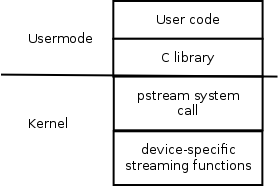
\includegraphics[width=0.5\textwidth]{stack.png}
	\end{center}
	\caption{The client-side streaming software stack}
	\label{figure:stack}
\end{figure}

The general structure of the streaming system on the client side is illustrated in Figure \ref{figure:stack}. At the top is user code, which calls functions in the C library. The library function {\tt stream} in turn calls the {\tt pstream} system call, which then deals with device-specific streaming functions based on which files are being accessed. On the server side is simply the 9P server, which is dealt with in the next chapter.

\section{The C Library}

The C library, also known as libc, provides an interface between user code and the kernel. It contains system calls such as {\tt read} and {\tt open} as well as a number of utility functions ({\tt strcmp}, {\tt dial}, \etc). The source for libc is located in {\tt /sys/src/libc} on Plan 9.

Files were added to the {\tt 9sys/} subdirectory to define the {\tt stream}, {\tt sclose}, {\tt sread}, and {\tt swrite} functions, described in the previous chapter. Since most of the complexity resides in the kernel, these functions turned out to be quite simple and are therefore reproduced in their entirety here.

\begin{program}
\begin{verbatim}
Stream*
stream(int fd, vlong offset, char isread) {
  Stream *s;
  s = mallocz(sizeof(Stream), 1);
  int r;

  s->addr = malloc(128);
  s->isread = isread;
  s->ofd = fd;
  s->offset = offset;
  r = pstream(fd, s->addr, offset, isread);
  if (r == -1) {
    // The server is not 9P2000.s compatible!
    s->compatibility = 1;
    return s;
  }
  if (s->addr == nil) {
    /* Error */
    return nil;
  }

  s->conn = dial(s->addr, 0, 0, 0);

  return s;
}
\end{verbatim}
\caption{The {\tt stream} function call}
\label{prog:stream}
\end{program}

The function in Program \ref{prog:stream}, {\tt stream}, serves to set up a stream. It initializes a Stream structure, then makes the {\tt pstream} system call. If the system call returns -1, the stream is set to compatibility mode; otherwise, the {\tt addr} member of the Stream struct will contain an IP address. If an IP address is returned, the {\tt stream} function calls {\tt dial} to make a new network connection to that address, which is then stored in the Stream structure; all future stream reads and writes then take place through this connection.

\begin{program}
\begin{verbatim}
long
swrite(Stream *s, void *buf, long len) {
  int n;

  if (s->isread == 0) {
    if (s->compatibility == 0)
      n = pwrite(s->conn, buf, len, -1LL);
    else
      n = pwrite(s->ofd, buf, len, s->offset);

    s->offset += n;
    return n;
  } else {
    return -1;
  }
}
\end{verbatim}
\caption{The {\tt swrite} function}
\label{prog:swrite}
\end{program}

\begin{program}
\begin{verbatim}
long
sread(Stream *s, void *buf, long len) {
  int n;

  if (s->isread == 1) {
    if (s->compatibility == 0)
      n = pread(s->conn, buf, len, -1LL);
    else
      n = pread(s->ofd, buf, len, s->offset);

    s->offset += n;
    return n;
  } else {
    return -1;
  }
}
\end{verbatim}
\caption{The {\tt sread} function}
\label{prog:sread}
\end{program}

The {\tt sread} and {\tt swrite} functions are nearly identical, the only difference being the use of {\tt pread} or {\tt pwrite}. As the functions show, if the compatibility bit is not set, data will be read from the TCP connection; otherwise, data will be read from the underlying file descriptor of the stream. Note that the offset is maintained in the Stream structure, allowing the stream to operate independently of any separate read or write calls issued on the file descriptor.

\begin{program}
\begin{verbatim}
int
sclose(Stream *s)
{
  if (!s->compatibility)
    close(s->conn);

  free(s->addr);
  free(s);
  return 0;
}
\end{verbatim}
\caption{The {\tt sclose} function}
\label{prog:sclose}
\end{program}

The task of the {\tt sclose} function is merely to simplify the process of closing a stream. It closes the TCP connection and then frees the previously-allocated memory regions as set up by the {\tt stream} function.

It was also necessary to modify several functions in the C library which convert 9P's struct representation to machine-independent messages and vice-versa. More specifically, cases were added to the {\tt convS2M}, {\tt convM2S}, and {\tt sizeS2M} functions to handle the new {\tt Tstream} and {\tt Rstream} messages.

\section{System Calls}

One system call was added to the kernel. This system call, {\tt pstream}, acts as an interface between the libc {\tt stream} function and the actual stream-setup functions in individual drivers. It takes as arguments a file descriptor, a buffer into which it should store a dial string, an offset, and the ``isread'' flag as passed to the {\tt stream} library call. It was necessary to add information about this system call to both the C library and the kernel itself.

The system call number for {\tt pstream}, number 52, was defined in the {\tt sys.h} header file. The function prototype for the system call was also defined in {\tt /sys/include/libc.h}. These were the only changes necessary to make libc aware of the existence of a new system call named {\tt pstream}.

Because the {\tt pstream} system call operates on files, its definition was placed in the {\tt sysfile.c} file in the kernel source. This file contains the implementations of system calls such as {\tt open}, {\tt read}, and {\tt write}. The {\tt syspstream} function, which was written to implement the behavior of the {\tt pstream} system call, parses the arguments given and converts the file descriptor to a channel. It then calls a device-specific {\tt stream} function based on the type of device to which the channel points.

\section{Device-specific Functions}

Each device must implement its own function to handle streams. However, in Plan 9, remote file systems are always connected to the local namespace using the {\tt devmnt} device; thus, to test the most important cases (high-latency Internet links), it was necessary to do a full implementation of streaming only for the {\tt devmnt} device. All other devices merely contain stub functions; these stub functions return -1, indicating that the device does not support streaming and that compatibility mode should be used.

\subsection{Devmnt}

The {\tt devmnt} device serves as an interface between the local namespace and 9P file systems. It converts read and write requests from multiple programs into 9P messages and multiplexes them over a single channel, which may be either a network connection or a local pipe.

To add streaming functionality to {\tt devmnt}, a new function, {\tt mntstream}, was written. This function is called by the {\tt pstream} system call to set up a new stream. When executed, it creates a new 9P request message of type {\tt Tstream}, which is then populated with the file descriptor of the desired file, the offset, and a flag indicating if the stream is read-type or write-type. It then transmits the 9P message to the server and waits for a reply.

When the reply is received, the incoming {\tt Rstream} message contains a string specifying an IP and port which can be connected to. However, {\tt devmnt} does not connect to the remote system itself; rather, it passes the dial string back up to the libc function {\tt stream}, which makes the connection.

\section{Compatibility Mode}

In designing and implementing streaming 9P, it was clear that not all 9P servers could be immediately modified to handle streaming, and that not all kernel devices were suited for streaming data. Thus it was necessary to design a compatibility mode, which would allow streaming-enabled programs to read data from a non-streaming server or device transparently.

The first step was the implementation of compatibility mode in the libc functions. When a stream is configured, the {\tt pstream} system call may return -1, specifying to the {\tt stream} function that streaming is not supported on the specified file. No error is raised, however. Instead, a flag is set in the Stream struct to designate the stream as requiring compatibility mode. Rather than reading from a network connection, {\tt sread} and {\tt swrite} read directly from the originally-specified file descriptor if a stream is set in compatibility mode. Although it offers no speed improvement, this allows programmers to use streams in their programs without the need for extensive error-checking and extra code.

At a lower level, the capability of a 9P server to stream is determined at the exchange of {\tt Tversion} and {\tt Rversion} messages. The {\tt devmnt} device, which handles connections to all non-kernel file systems, identifies itself as speaking the {\tt 9P2000.s} protocol. The definition of the {\tt Tversion} message means that {\tt 9P2000.s} is compatible with {\tt 9P2000}, so non-streaming servers accept this version and report back as speaking {\tt 9P2000}. However, streaming servers will also answer with {\tt 9P2000.s}. When the {\tt mntstream} function is later called to set up a stream, the version reported by the server is checked. If the server reported its version as {\tt 9P2000}, compatibility mode is used; if it reported {\tt 9P2000.s}, a {\tt Tstream} message is sent to establish a stream.

\section{Organization Overview}

Figure \ref{figure:flowchart}, on the following page, shows a high-level view of the way a stream is configured. Different levels of implementation are indicated in different colors. 

As the flowchart shows, a user program calls the {\tt stream} function, giving it a file descriptor and other arguments. In turn, {\tt stream} calls the {\tt pstream} system call, passing along the appropriate arguments. The {\tt pstream} system call does little more than call the device-appropriate streaming function based on the location of the selected file--in the case of the example in the flowchart, {\tt mntstream}.

The {\tt mntstream} function checks if the remote server supports streaming. If the server does not support streaming, {\tt mntstream} returns -1. The -1 return value is passed back up through {\tt pstream} to {\tt stream}, which configures the stream structure in compatibility mode and returns.

If, on the other hand, the server supports streaming, {\tt mntstream} sends a {\tt Tstream} message to the server requesting a new stream. The server in turn prepares a TCP port for the file transfer and replies with an {\tt Rstream} message. When it receives the reply, {\tt mntstream} extracts the given IP and port number, then returns to {\tt pstream}, which returns to {\tt stream}. {\tt stream} then connects to the server, which begins reading from the connection or sending data over it, depending on the stream type. At this point, the {\tt stream} function returns to the user program and the stream is ready to be used.

\begin{figure}[h]
	\begin{center}
		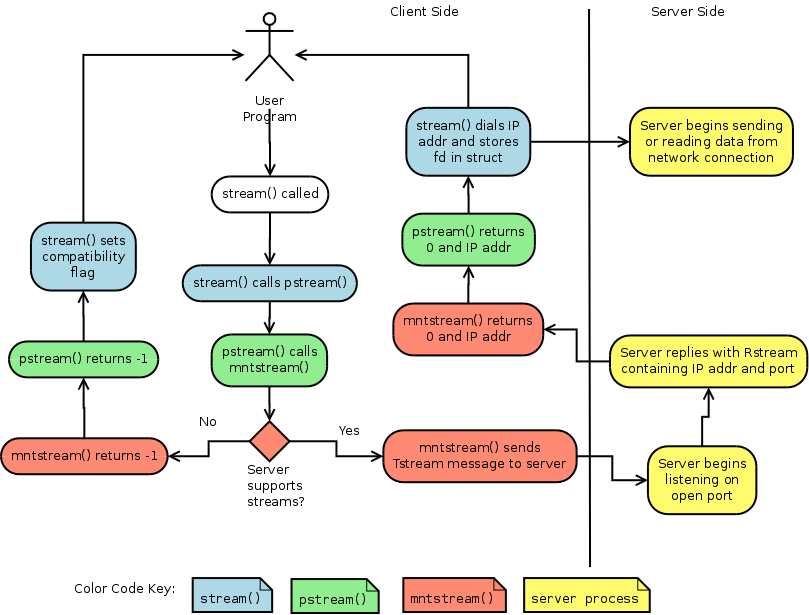
\includegraphics[width=1\textwidth]{flowchart.png}
	\end{center}
	\caption{Streaming organization flowchart}
	\label{figure:flowchart}
\end{figure}

\section{Summary}

This chapter described the implementation of streaming in Plan 9 and the 9P protocol, from the kernel level to the C library functions used by programmers. The next chapter describes the methods for modifying existing programs and file servers to take advantage of streams.

\chapter{Modifying Existing Programs}

Streams are used by regular user programs (such as {\tt cp}) and by 9P servers (such as {\tt exportfs}, which serves the namespace of a CPU server). The functions described in the previous section are utilized by these programs to request and use streams. In order to test the newly-implemented streaming capabilities, the {\tt cp} command and the {\tt exportfs} file server were both modified in order to accept streams; their specific changes are described after the general section.

\section{General Modification Practices}

There are two classes of programs which must be modified to use streams: user programs (clients) and 9P servers. A separate strategy is needed for each different type of program, but the same general practices should be applicable to nearly all cases.

In modifying user programs, the process is extremely simple. The programmer must first identify places where the program accesses a file sequentially. Then, after the file is opened using the {\tt open} function, the programmer inserts a call to the {\tt stream} function requesting a read or write stream, as appropriate. After the stream is established, existing {\tt read} or {\tt write} calls are changed to {\tt sread} and {\tt swrite} calls. Finally, when the stream is no longer needed, the {\tt sclose} function is called to shut down the stream.

Modifying 9P servers is more complex, but not excessively so. Although the design can vary, in general a 9P server has a function to accept incoming 9P messages and call an appropriate handler function to reply. A new handler function must be added to reply to stream requests. The function should begin listening on a random open port, then create a {\tt Rstream} message containing the IP and port number and send the reply to the client. It then must wait for a connection on that port; when the connection is established, it begins either reading from or writing to that TCP connection from the appropriate file. The handler function should be launched by the server as a separate process to allow further 9P messages to be processed.

\section{cp}

In Plan 9, {\tt cp} is a very simple program. Before modification, it simply opened the source and destination files, then read 8 KB at a time from the source and wrote it to the destination. This proved to be very simple to rewrite for streaming. First, calls to {\tt stream} were added after the source and destination files were opened. Then, the calls to {\tt read} and {\tt write} were simply replaced by equivalent calls to {\tt sread} and {\tt swrite}. Thanks to streaming compatibility mode, it was possible to make these changes to {\tt cp} and still access files from non-streaming sources without any special knowledge on the part of the programmer.

\section{exportfs}

The {\tt exportfs} file server provides an external interface to the namespace of a CPU server. It was chosen for modification due to its simplicity.

The basic structure of {\tt exportfs} is this: It listens on a specific port for incoming connections. When an incoming connection is established, the server then forks a process to listen on that connection for incoming 9P messages. As messages come in, their message types are used to select an appropriate handler function. In the case of the {\tt Topen}, {\tt Tread}, and {\tt Twrite} messages, which are likely to take longer, the handler function is called {\tt slave}. This function and its sub-fuction {\tt blockingslave} fork a separate process for each message to prepare a response while the main thread continues to reply to other messages. The new process then enters a message-specific function handler to make its response.

Given that streaming a file may require a very long time (in the case of a 2 gigabyte file, for example), it was clear that the handler should be forked as a separate process, similar to that of {\tt Tread} or {\tt Twrite}. To that end, the {\tt blockingslave} function was modified so that in the case of a {\tt Tstream} message, the {\tt slavestream} function would be executed in a new process.

The {\tt slavestream} function was a modification of the existing {\tt slaveread} function. When called, it begins listening on a random, unused TCP port. It then takes the IP address of the server and the port on which it is listening and places them into the data field of the {\tt Rstream} reply message, which it then transmits. Having told the client where to connect, {\tt slavestream} then waits for a connection on the specified port. Once the connection is made, it enters a loop. Depending on whether the stream type is read or write, it either reads from the selected file and writes to the TCP connection (in the case of a read stream), or reads from the TCP connection and writes to the selected file (in the case of write). If it is a read stream, the loop ends when the source file has been fully read and transmitted. In the case of a write stream, the loop ends when the client closes the TCP connection, signaling the end of the stream.

\chapter{Results}

Having implemented streaming functionality in the Plan 9 system, it was necessary once again to run tests and compare the results to those gathered before. Using the modified {\tt exportfs} and {\tt cp} programs, described in the previous chapter, several different files were transferred over the network at varying latencies.

The same network setup used for initial testing (Figure \ref{figure:network2}) was re-used to test streaming 9P. Specifically, the client computer (named ``illiac'') was an IBM Thinkpad T22 laptop with a Pentium III processor and 512 MB of RAM running a streaming-enabled Plan 9 terminal kernel; it used the laptop's local hard drive as the filesystem root. The server (named ``p9'') had dual Pentium III processors and 1 GB of RAM running a stock Plan 9 cpu/auth/fileserver kernel. The configuration of the server was changed to use the modified {\tt exportfs} executable; otherwise, no special changes were necessary. The server also ran the Plan 9 HTTP server.

\section{Transfer Speed Test}

As before, the same set of randomly-generated 10 MB, 50 MB, 100 MB, and 200 MB files were transferred over the network with round-trip latencies of 500 $\mu$s, 15 ms, and 50 ms. Each file was transferred five times; the mean transfer times and the associated standard deviations are shown in the results tables. On the client computer, the server's namespace was mounted using the command {\tt import p9 / /n/p9}, which mounted the server's root directory to the local directory {\tt /n/p9}; the {\tt import} command specifically connected to the {\tt exportfs} service running on the server.

In order to transfer a file from the server to the client using the streaming copy program, {\tt scp}, a command such as {\footnotesize {\tt scp /n/p9/usr/john/random10M /dev/null}} was used. Similarly, the command {\footnotesize{\tt cp /n/p9/usr/john/random10M /dev/null}} was used to transfer the same file using the non-streaming copy program. To transfer the files using HTTP, the {\tt hget} program was utilized, with the command line {\footnotesize{\tt hget http://p9/random10M > /dev/null}} fetching the remote file and directing the output to the null device. The times were gathered using the Plan 9 {\tt time} command (also present in Unix), which reports the elapsed time required to complete the execution of a program.

\begin{figure}[h]
	\begin{center}
		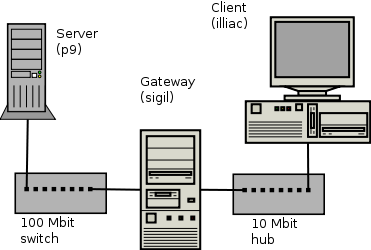
\includegraphics[width=0.75\textwidth]{network.png}
	\end{center}
	\caption{Network for simulating artificial latency}
	\label{figure:network2}
\end{figure}

Table \ref{table:nolatency2} and Figure \ref{figure:nolatency2} show the resulting transfer times when no artificial latency was induced (average round-trip time 500 $\mu$s). At such a low latency, 9P, streaming 9P, and HTTP all performed approximately the same, with streaming 9P and HTTP within a standard deviation of each other. One interesting result from these tests is the performance of 9P vs. HTTP and streaming 9P as the file sizes increase. For small file sizes, over the low latency connection, 9P outperformed HTTP and streaming 9P. However, when the file sizes rose past 100 MB, streaming 9P and HTTP were faster than regular 9P. This indicates that the additional time required to set up a separate stream and the slight overhead incurred by the {\tt sread} and {\tt swrite} functions may make streaming slightly less efficient than regular 9P when transferring small files over low-latency connections.

\begin{table}[h]
	\caption{HTTP vs. 9P vs. Streaming 9P, no induced latency, average RTT 500 $\mu$s}
	\begin{center}
		\begin{tabular}{ | c || c | c | c | c | c | c | }
			\hline
			& \multicolumn{2}{| c |}{\bf{9P (sec.)}} & \multicolumn{2}{| c |}{\bf{HTTP (sec.)}} & \multicolumn{2}{| c |}{\bf{Streaming 9P}}\\ \hline
			\bf{File Size (MB)} & \bf{mean} & \bf{std. dev.} & \bf{mean} & \bf{std. dev.} & \bf{mean} & \bf{std. dev.} \\ \hline
			10 & 10.91 & 0.51 & 12.66 & 0.37 & 12.71 & 0.31 \\ \hline
			50 & 59.21 & 2.34 & 62.75 & 0.33 & 62.11 & 0.29 \\ \hline
			100 & 126.96 & 5.72 & 125.30 & 0.58 & 125.58 & 0.58 \\ \hline
			200 & 262.40 & 0.37 & 251.41 & 0.59 & 251.53 & 0.87 \\ \hline
		\end{tabular}
	\end{center}
	\label{table:nolatency2}
\end{table}

\begin{figure}[h]
	\begin{center}
		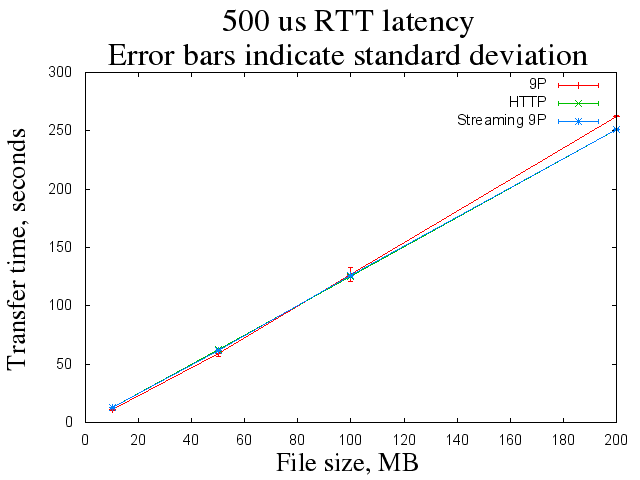
\includegraphics[width=0.75\textwidth]{results/res2/500us.png}
	\end{center}
	\caption{HTTP vs. 9P vs. Streaming 9P, 500 $\mu$s RTT}
	\label{figure:nolatency2}
\end{figure}

When the latency was increased to 15 ms round-trip, as shown in Table \ref{table:15ms2} and Figure \ref{figure:15ms2}, regular 9P immediately fell significantly behind HTTP, while streaming 9P maintained almost exactly the same performance as HTTP. Differences between the transfer speeds of the two protocols were small enough to be considered mere experimental variance.

\begin{table}[h]
	\caption{HTTP vs. 9P vs. Streaming 9P, Average RTT 15 ms}
	\begin{center}
		\begin{tabular}{ | c || c | c | c | c | c | c | }
			\hline
			& \multicolumn{2}{| c |}{\bf{9P (sec.)}} & \multicolumn{2}{| c |}{\bf{HTTP (sec.)}} & \multicolumn{2}{| c |}{\bf{Streaming 9P}}\\ \hline
			\bf{File Size (MB)} & \bf{mean} & \bf{std. dev.} & \bf{mean} & \bf{std. dev.} & \bf{mean} & \bf{std. dev.} \\ \hline
			10 & 30.85 & 1.34 & 14.47 & 0.55 & 14.41 & 0.11 \\ \hline
			50 & 156.29 & 2.84 & 71.41 & 0.41 & 70.91 & 0.51 \\ \hline
			100 & 319.88 & 5.8 & 144.44 & 0.50 & 142.10 & 1.07 \\ \hline
			200 & 647.22 & 1.87 & 286.56 & 2.06 & 284.60 & 0.61 \\ \hline
		\end{tabular}
	\end{center}
	\label{table:15ms2}
\end{table}

\begin{figure}[h]
	\begin{center}
		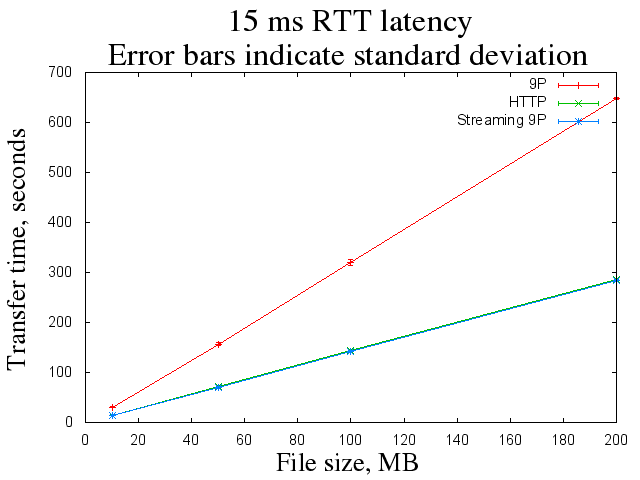
\includegraphics[width=0.75\textwidth]{results/res2/15ms.png}
	\end{center}
	\caption{HTTP vs. 9P vs. Streaming 9P, 15 ms RTT}
	\label{figure:15ms2}
\end{figure}

Figure \ref{figure:50ms2} and Table \ref{table:50ms2} show the results at 50 ms induced round-trip latency. As in the previous test, streaming 9P and HTTP took almost exactly the same amount of time to transfer the same data, remaining within a standard deviation of each other.

\begin{table}[h]
	\caption{HTTP vs. 9P vs. Streaming 9P, 50 ms RTT}
	\begin{center}
		\begin{tabular}{ | c || c | c | c | c | c | c | }
			\hline
			& \multicolumn{2}{| c |}{\bf{9P (sec.)}} & \multicolumn{2}{| c |}{\bf{HTTP (sec.)}} & \multicolumn{2}{| c |}{\bf{Streaming 9P}}\\ \hline
			\bf{File Size (MB)} & \bf{mean} & \bf{std. dev.} & \bf{mean} & \bf{std. dev.} & \bf{mean} & \bf{std. dev.} \\ \hline
			10 & 75.15 & 0.41 & 19.58 & 0.23 & 19.88 & 0.12 \\ \hline
			50 & 379.67 & 2.04 & 96.71 & 0.46 & 96.83 & 0.66 \\ \hline
			100 & 767.93 & 5.19 & 193.10 & 1.40 & 193.23 & 0.58 \\ \hline
			200 & 1543.12 & 0.62 & 385.292 & 1.85 & 386.02 & 1.77 \\ \hline
		\end{tabular}
	\end{center}
	\label{table:50ms2}
\end{table}

\begin{figure}[h]
	\begin{center}
		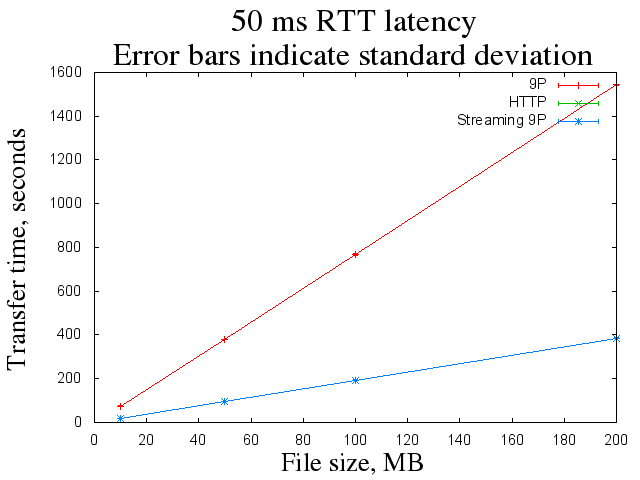
\includegraphics[width=0.75\textwidth]{results/res2/50ms.png}
	\end{center}
	\caption{HTTP vs. 9P vs. Streaming 9P, 50 ms RTT}
	\label{figure:50ms2}
\end{figure}

The results cited above clearly show that streaming 9P is competitive with HTTP and can easily outperform regular 9P. Indeed, when the standard deviations of the tests involved are considered, it is fair to say that HTTP and 9P experienced essentially the same performance. The results also show that the addition of streaming does not cause any loss of performance over low-latency links, an especially important consideration in the context of supercomputing specifically and local networking in general.

Since it is quite likely that multiple programs may stream files at the same time, another test was performed to compare the scalability of streaming 9P.

\section{Concurrency Test}

In order to test the performance of multiple programs streaming files simultaneously, the previous test was repeated ``concurrently''. The commands which had previously been issued one at a time, for example {\footnotesize{\tt time cp /n/p9/usr/john/random10M /dev/null}}, were followed by a {\tt \&} character, which caused the command to be executed in the background and allowed for the execution of multiple client programs at the same time.

Tests were performed using two, four, and eight simultaneous client programs on the client PC. For the test, a round-trip latency time of 50 milliseconds was used with a file size of 10 MB. The execution times for each instance of the programs were averaged to get the results shown in Table \ref{table:concurrent} and Figure \ref{figure:concurrent}.

\begin{table}[h]
	\caption{10 MB file transfer speeds with multiple concurrent clients}
	\begin{center}
		\begin{tabular}{ | c || c | c | c |}
			\hline
			\bf{Number of Clients} & \bf{Streaming 9P (sec.)} & \bf{HTTP (sec.)} & \bf{9P (sec.)} \\ \hline
			2 & 30.96 & 28.51 & 79.75 \\ \hline
			4 & 53.28 & 52.53 & 100.81 \\ \hline
			8 & 104.24 & 101.93 & 158.53 \\ \hline
		\end{tabular}
	\end{center}
	\label{table:concurrent}
\end{table}

\begin{figure}[h]
	\begin{center}
		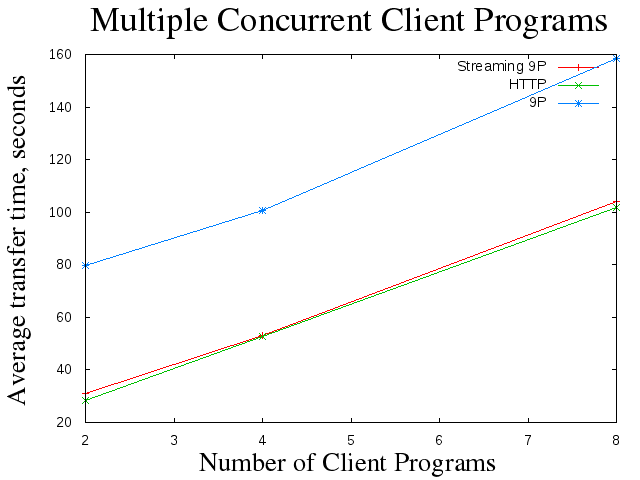
\includegraphics[width=0.75\textwidth]{results/concurrent.png}
	\end{center}
	\caption{10 MB file transfer speeds with multiple concurrent clients}
	\label{figure:concurrent}
\end{figure}

As the results show, all three protocols experienced increased transfer times as the number of concurrent transfers increased. Streaming 9P and HTTP both showed approximately the same level of scalability within the limited confines of this test, with performance decreasing in a slow and linear fashion.

%  A citation~\cite{CrammingMoreComponentsOntoIntegratedCircuits}...
%A glossary entry~\gloss{Term} used in the text.
%Another glossary entry~\gloss{RIT} used in the text.

\chapter{Conclusions}

\section{Conclusions}
As initially stated, the existing 9P file protocol experiences poor file transfer performance over high latency network connections, which are common on the Internet. When transferring over a typical Internet connection, 9P often takes several times as long as HTTP. The problem exists because of the design of 9P; to read data, a request message is sent by the client, which must then wait the entire round-trip time of the connection to receive the data in a response message. This induces a long wait every time a program wishes to read or write data. The HTTP and FTP protocols are focused specifically on reading and writing files sequentially, a very common access case. 9P, on the other hand, provides no concessions to the sequential file access method.

In order to correct the latency problem, this work proposed a separate method for sequentially reading or writing files called streaming. The streaming operations augment the existing POSIX-style file I/O operations, such as opening or reading a file, with additional operations designed specifically for sequentially reading or writing files. This streaming functionality was implemented in 9P by using in-band protocol messages to negotiate an out-of-band TCP connection for transferring file data. This method of operation mimics that of FTP in passive mode. Specifically, the client computer sends a {\tt Tstream} message to the server, which responds with an {\tt Rstream} message containing an IP address and TCP port. The client then connects to that IP and port and either reads a file or writes out data over the TCP connection. By adding streaming functionality to 9P, this work:

\begin{itemize}
	\item Extended Plan 9's file operations to specifically include sequential file operations
	\item Allowed files to be transferred at speeds comparable to HTTP and FTP
	\item Presented ways in which existing programs may be easily modified to use the new functionality
\end{itemize}

Modifications were inserted at all levels of the Plan 9 system, including new C library functions, a new system call, and additional handler functions in kernel devices. The end result was a simple system which allows programmers to read and write files sequentially using streams with minimal program modifications. Using the {\tt stream} library function, client programs request a read stream or a write stream, then read or write data from or to that stream using the {\tt sread} or {\tt swrite} functions before finally closing the stream with the {\tt sclose} function. In turn, 9P file servers implement additional functionality to understand the stream initialization 

Experimental results were promising. File transfer times using 9P were found to be comparable with those of HTTP when used over high latency links. At the same time, no degradation in performance was found when using streams over low latency (local) connections. Additionally, tests with multiple programs streaming simultaneously indicated that streaming 9P was approximately as scalable as HTTP, with a slow loss in performance as the number of client programs increased.

The experimental implementation demonstrated in this document appears to be reasonably strong. With the implementation of ``compatibility mode,'' programs using the new streaming extensions may access files on non-streaming servers transparently. Although true streaming currently occurs only when a file resides on a remote system, there is no need for the programmer to distinguish between local and remote files; as with the rest of Plan 9, the actual physical location of the file is immaterial to the user.

The new streaming 9P extensions stand to improve significantly the quality of user experience in the Plan 9 system. By allowing 9P to compete with HTTP for file transfers over high-latency connections, the usability of the protocol is enhanced at little to no cost to the end users and programmers. The addition of streaming to 9P may also prove useful in supercomputing applications, where large files are routinely transferred; although the latencies involved are small, the use of streaming could reduce network overhead by replacing repeated {\tt Tread}/{\tt Rread} messages with simple TCP connections.

\section{Future Work}
Future work in this area would begin with the conversion of more file servers and user programs to use streams. Any file server which is commonly accessed over a network connection (rather than locally through a system pipe) would benefit from the addition of streaming capability. Specifically, the disk-backed file servers Fossil and Venti are ideal targets for streaming. When a Plan 9 system such as a terminal mounts a root file system, it typically connects to a remote Fossil server; providing streaming within Fossil would allow users to experience more efficient file accesses in almost all of their files.

The image and document viewers could benefit from streaming file accesses, since they often read large files sequentially. The MP3 decoder is another obvious client program that could use streams, since it must be able to access file data quickly enough to continue playing without pausing. As the introduction chapter explains, playing MP3 files with 9P over the Internet causes skipping in playback; using streams should eliminate that problem.

Additionally, it may be advantageous to modify other kernel devices (beyond the already-modified {\tt devmnt}) to support streaming; for example, the audio device may benefit from the use of streams. Testing would be required to determine if such a modification is feasible or useful.


  \nocite{*}
%%%%%%%%%%%%%%%%%%%%%%%%%%%%%%%%%%%%%%%%%%%%%%%%%%%%%%%%%%%%%%%%%%%%%%%%%%%%%%%

%%%%%%%%%%%%%%%%%%%%%%%%%%%%%%%%%%%%%%%%%%%%%%%%%%%%%%%%%%%%%%%%%%%%%%%%%%%%%%%
\bibliographystyle{plain}
% Single space the bibliography to save space.
\begin{singlespace}
\bibliography{Thesis}
\end{singlespace}
%%%%%%%%%%%%%%%%%%%%%%%%%%%%%%%%%%%%%%%%%%%%%%%%%%%%%%%%%%%%%%%%%%%%%%%%%%%%%%%

%%%%%%%%%%%%%%%%%%%%%%%%%%%%%%%%%%%%%%%%%%%%%%%%%%%%%%%%%%%%%%%%%%%%%%%%%%%%%%%
% The appendices are (of course) optional.
%\appendix
%\chapter{A Long Proof}
%  ...
%%%%%%%%%%%%%%%%%%%%%%%%%%%%%%%%%%%%%%%%%%%%%%%%%%%%%%%%%%%%%%%%%%%%%%%%%%%%%%%
\end{document}
